\subsection{Stabilità dello spettrometro}

Facciamo una misura lunga circa 20 ore con la sorgente a \SI{70}{\degree} senza bersaglio per valutare la stabilità in risposta dello spettrometro (ovvero il sistema rivelatore-preampli-ampli-ADC).
La scelta dell'angolo è forzata dal rate di campionamento massimo (\SI{40}{Hz}) dell'ADC.

Mostriamo in \autoref{stab} i valori campionati in funzione del tempo. Non osserviamo nessuna variazione di energia rispetto ad una misura di breve durata.

\begin{figure}[h]
\centering
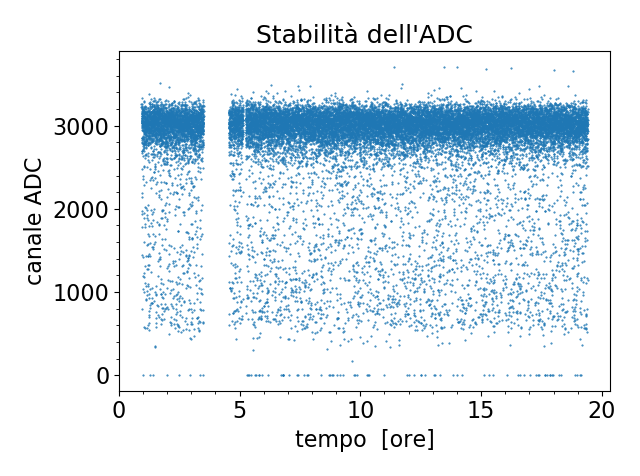
\includegraphics[width=30 em]{immagini/stab.png}
\caption{Valori acquisiti in funzione del tempo. Gli spazi vuoti tra una serie di dati e l'altra vengono dal fatto che sono state unite 4 acquisizioni quasi consecutive.
In questo grafico è presente soltanto un punto ogni 100 perché la rappresentazione completa rendeva illeggibile la figura.}
\label{stab}
\end{figure}

Guardando l'istogramma di questi dati ci siamo accorti che l'ADC presenta degli accumuli nei canali corrispondenti alle varie potenze di 2. Questo accade quando in un numero binario vengono cambiate più cifre alla volta, cosa che si verifica quando si raggiungono le varie potenze di 2. L'ADC impiega più tempo a cambiare valore e la misura successiva rimane nel bin precedente.
Per aggirare questo problema ribinniamo i dati usando dei bin che abbiano come bordi (0,32]+32n, dove n è un intero. Mostriamo questo effetto in \autoref{picchi} insieme alla sua ``correzione''.

\begin{figure}[h]
\centering
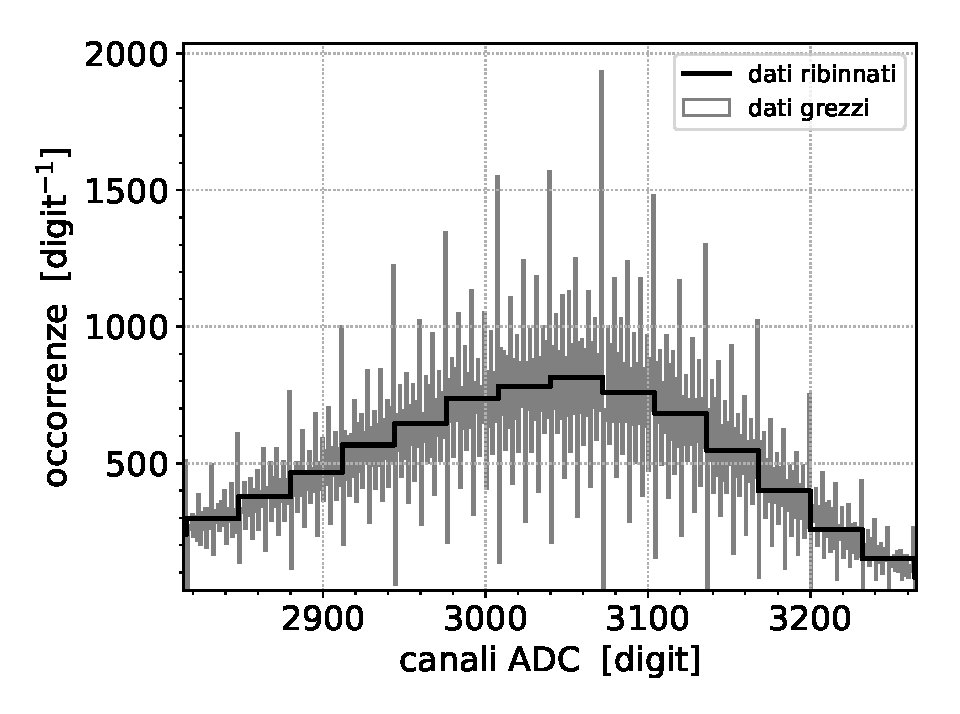
\includegraphics[width=30 em]{immagini/rebin}
\caption{Istogramma di una parte dei dati della misura di stabilità in cui si vedono gli accumuli a cui è soggetta l'ADC e la nostra soluzione.}
\label{picchi}
\end{figure}